\section{Введение}
Первая лабораторная работа. Номер работы 1a

От генератора сигналов на частотомер подается последовательность
трапецеидальных импульсов, параметры которых задаются преподавателем.
Задаваемый период следования импульсов измеряется с помощью
частотомера на двух шкалах: грубой и точной. В качестве генератора
импульсов используется генератор Г5-2А (или ему подобный), а в качестве
частотомера – Ч3-32 (или того же типа).

\subsection{Цель работы}

Научится правильно оценивать получившиеся в ходе эксперимента результаты

\subsection{Решаемые задачи}

Измерение электронным частотомером Ч3-32 периода следования импульсов, задаваемых на выходе генератора.

Оценка результатов эксперимента.

\section{Основная часть}

\subsection{Теоретическая часть}

Предоставленая формула для оценки погрешности прибора, взята из паспорта прибора: 

\begin{equation}
    \gamma=\pm(\gamma_0 +\frac{1}{f_x T})*100\%
    \label{error:tool_source}
\end{equation}
где $f_x$ -- измеряемая величина, $T$ -- период следования импульсов ($1$ для грубой шкалы, $0.1$ для точной), $\gamma_0$ константа равная $5*10^{-7}$.

Учитывая что $\gamma = \frac{\delta f_x}{f_x}*100\%$, после преобразований формула приймет вид
\begin{equation}
    \delta f_x = \frac{1}{f_x} + 5 * 10^{-7} f_x
    \label{error:tool_trans}
\end{equation}

Фомулы для погрешности измерений, взяты из присланых материалов:

\begin{equation}
    \overline{f} = \frac{\sum f}{N}, 
    s_{\overline{f}} = \sqrt{\frac{\sum f-\overline{f}}{N (N-1)}}, 
    \delta f = s_{\overline{f}} * t(\alpha, N)
    \label{eq:binom5}
\end{equation}

\subsection{Эксперимент}
Преподаватель подключает все в сеть.

Выполняем 10 измерений на грубой шкале. Получившаяся погрешность нас не устраивает, т. к. погрешность прибора и случайная погрешность измерения лежат достаточно близко и неудобно считать итоговую погрешность. 

Переходим к измерениям на точной шкале. Выполняем 50 измерений на точной шкале.

\begin{figure}[ht!]
\centering
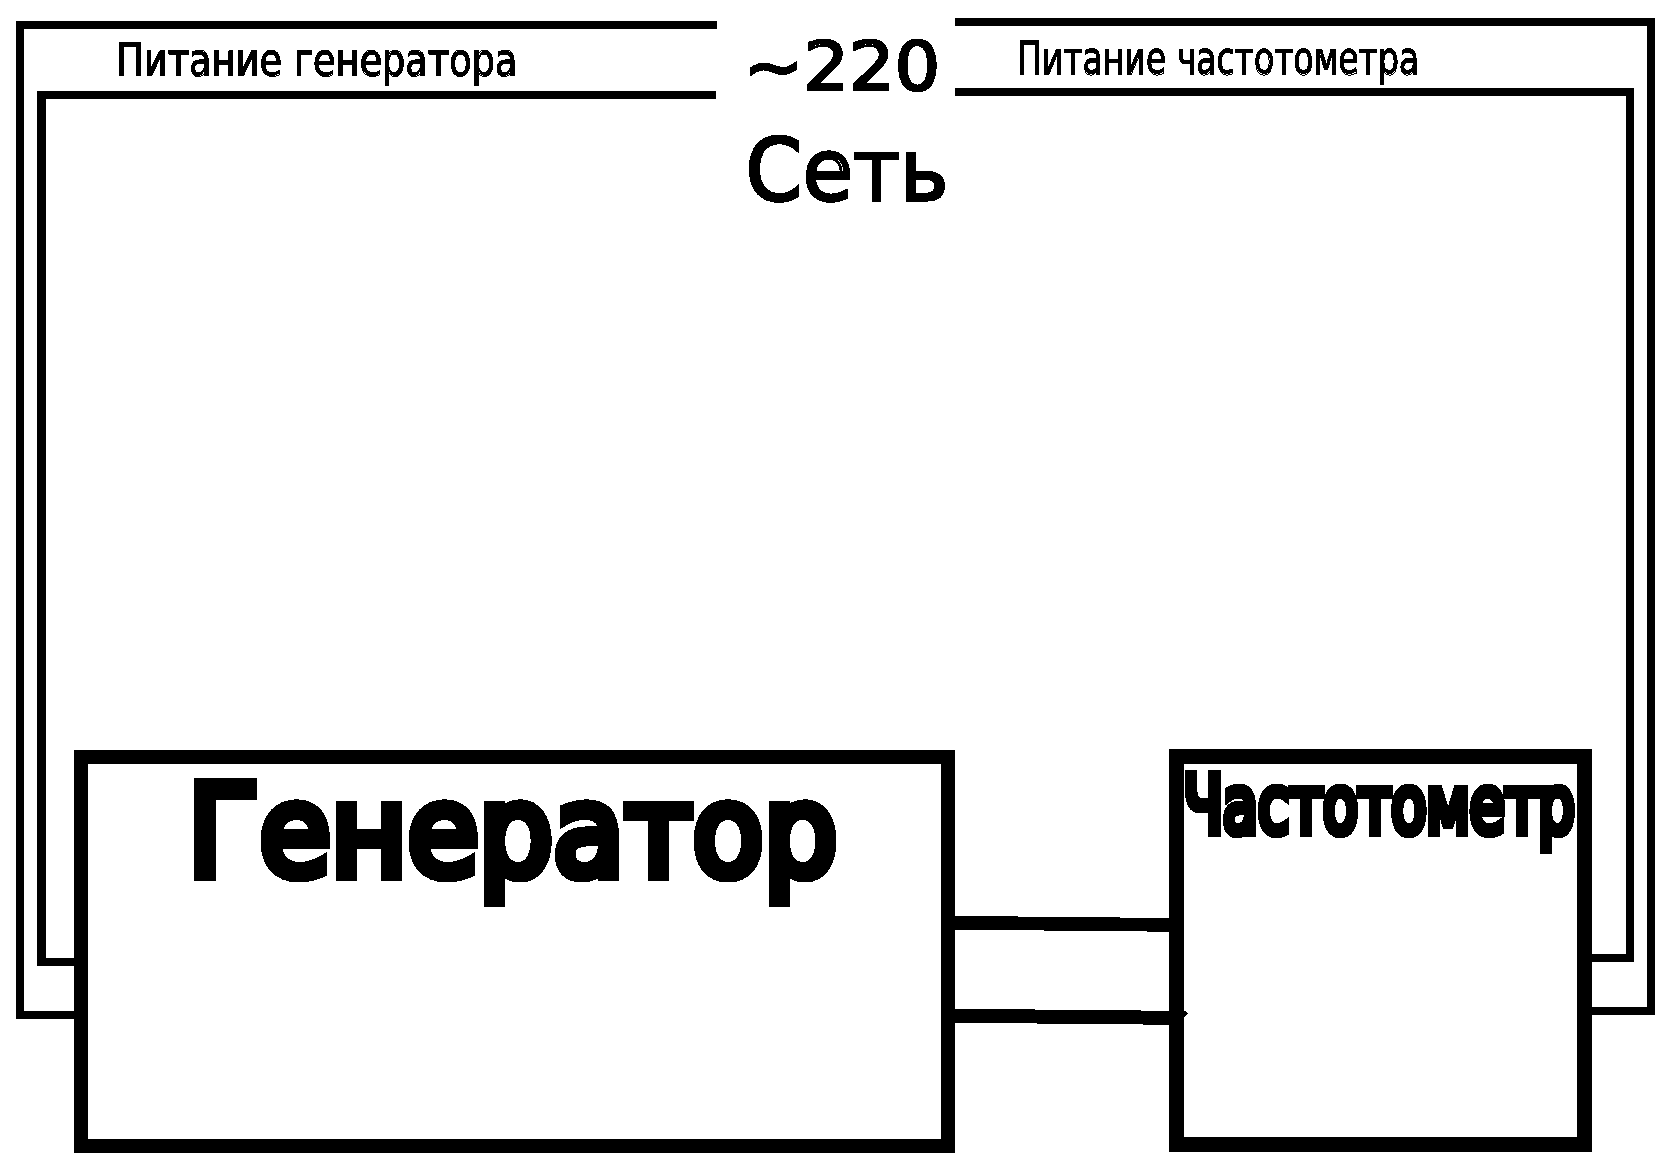
\includegraphics[width=0.8\textwidth]{scheme.eps}
\caption{Схема установки}
\label{fig:sketch}
\end{figure}

\subsection{Обработка данных и обсуждение результатов}

После переноса результатов в csv файл, написана програма на c++ для обработки результатов.

Для точной шкалы:

среднее значение: 4610 Гц

случайная погрешность: 2.6 Гц

погрешность прибора: 1.1 Гц

Ошибка прибора мала по сравнению со случайной погрешностью, поэтому можем говорить что полная погрешность это 2.6Гц

\subsubsection{Исходный код}
Пояснени по расчету коэфициенов Студента

\begin{lstlisting}[label=listing1, caption=Рачет коэфициента Студента]
private:
  static double student_coef(size_t n, double alpha) {
    if (n <= 1) {
      return 0.0;
    }
    boost::math::students_t dist(n - 1);
    /*
     *                     alpha
     <----|--------------------------------------|---->
        -t_stat              0                 +t_stat
    */
    auto t_stat = boost::math::quantile(dist, 0.5 + alpha / 2.0);
    return t_stat;
  }
\end{lstlisting}

\subsubsection{Таблицы}
Таблицы с имерениями см. Таблица~\ref{tabl:1}), Таблица~\ref{tabl:2}).

\begin{table}[ht!]
\centering
\caption{Измерения на грубой шкале}
\label{tabl:1}
\begin{tabular}{|c|c|c|c|}
\hline
\begin{minipage}{3cm}
    Номер п.п.
\end{minipage} &
\begin{minipage}{4cm}
    Диапазон показаний использованной шкалы прибора (кГц)
\end{minipage} &
\begin{minipage}{4cm}
    Результаты отдельных наблюдений ($f_i$) (кГц)
\end{minipage} &
\begin{minipage}{4cm}
    Погрешность прибора на данной шкале ($\Delta f_{\text{приб}}$) (кГц)
\end{minipage} \\ \cline{1-4}
1  & \multirow{10}{*}{$0 - 10^5$} & 4,68 & 0,01 \\ \cline{1-1} \cline{3-4}
2  & & 4,60 & 0,01 \\ \cline{1-1} \cline{3-4}
3  & & 4,62 & 0,01 \\ \cline{1-1} \cline{3-4}
4  & & 4,60 & 0,01 \\ \cline{1-1} \cline{3-4}
5  & & 4,62 & 0,01 \\ \cline{1-1} \cline{3-4}
6  & & 4,60 & 0,01 \\ \cline{1-1} \cline{3-4}
7  & & 4,60 & 0,01 \\ \cline{1-1} \cline{3-4}
8  & & 4,60 & 0,01 \\ \cline{1-1} \cline{3-4}
9  & & 4,62 & 0,01 \\ \cline{1-1} \cline{3-4}
10 & & 4,60 & 0,01 \\ \hline
\end{tabular}
\end{table}

\csvreader[
    longtable=|c|c|c|c|, % Заменяет tabular, определяет границы
    separator=semicolon,
    table head={
        \caption{Измерения на точной шкале} \label{tabl:2} \\ \hline
        \multirow{2}{*}{№ п.п.} &
        \begin{minipage}{5cm}
            Результат наблюдений ($f_i$)
        \end{minipage} &
        \begin{minipage}{5cm}
            Случайные отклонение от среднего $d_i=f_i-\overline{f}$
        \end{minipage} &
        \begin{minipage}{5cm}
            $d_i^2=(f_i-\overline{f})^2$
        \end{minipage} \\ \cline{2-4}
        & кГц & кГц & кГц \\ \hline
        \endfirsthead % Конец заголовка первой страницы
        
        \multicolumn{4}{c}{Продолжение таблицы \ref{tabl:2}} \\ \hline 
        {№ п.п.} &
        \begin{minipage}{5cm}
            Результат наблюдений ($f_i$)
        \end{minipage} &
        \begin{minipage}{5cm}
            Случайные отклонение от среднего $d_i=f_i-\overline{f}$
        \end{minipage} &
        \begin{minipage}{5cm}
            $d_i^2=(f_i-\overline{f})^2$
        \end{minipage} \\ \hline
        \endhead % Конец заголовка для всех последующих страниц
    },
    late after line={\\ \hline}
]{lab_table.csv}{
    N=\colN, 
    {Source KHz}=\colSource, 
    {d kHz}=\cold, 
    {d_squre kHz}=\colsq
}{
    \colN & \colSource & \cold & \colsq
}

\subsubsection{Графики}

По результатам эксперимента пстроены графики \ref{fig:plot} \ref{fig:gistogram}
\begin{figure}[ht!]
\centering
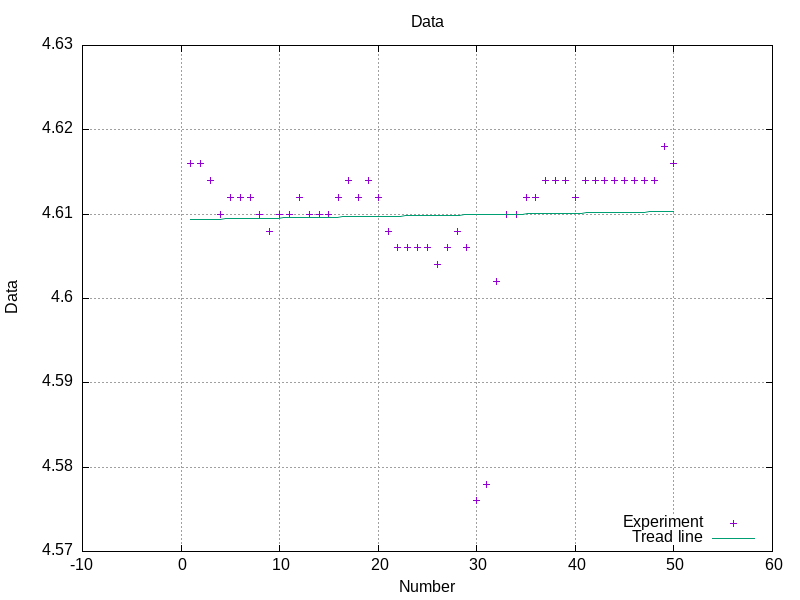
\includegraphics[width=0.8\textwidth]{plot_data.png}
\caption{Распределение измерений для точной шкалы}
\label{fig:plot}
\end{figure}

\begin{figure}[ht!]
\centering
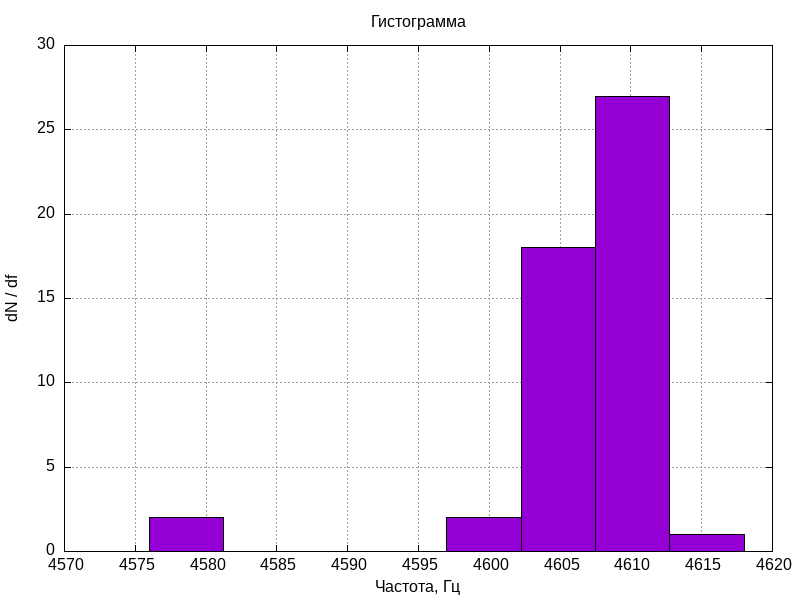
\includegraphics[width=0.8\textwidth]{gistogram.png}
\caption{Гистограма измерений для точной шкалы}
\label{fig:gistogram}
\end{figure}


\section{Выводы}

Ответ $4610 \pm 3$ Гц 
Экспереминт поставлен хорошо, погрешность достаточно мала по сравнению с измерямой величиной.
% Никаких выводов очев